\documentclass[12pt]{article}

\usepackage{sbc-template}
\usepackage{graphicx, url}
\usepackage[utf8]{inputenc}
\usepackage[brazil]{babel}
\usepackage{url}
\newcommand{\aspas}[1]{``#1''} % Comando para colocar aspas em um texto
\usepackage{setspace} % Para determinar o espaçamento entre linhas
\usepackage{float} % Usado para posicionamento de imagens
\usepackage{svg}
\usepackage{array} % Para ajustar tabelas
\usepackage{listings} % Para inserir código fonte na página
\usepackage{xcolor}

\definecolor{codegreen}{rgb}{0,0.6,0}
\definecolor{codegray}{rgb}{0.5,0.5,0.5}
\definecolor{codepurple}{rgb}{0.58,0,0.82}
\definecolor{backcolour}{rgb}{0.95,0.95,0.92}

\lstdefinestyle{mystyle}{
	backgroundcolor=\color{backcolour},   
	commentstyle=\color{codegreen},
	keywordstyle=\color{magenta},
	%	numberstyle=\tiny\color{codegray},
	stringstyle=\color{codepurple},
	basicstyle=\ttfamily\footnotesize,
	breakatwhitespace=false,         
	breaklines=true,                 
	captionpos=b,                    
	keepspaces=true,                 
	%	numbers=left,                    
	%	numbersep=5pt,                  
	showspaces=false,                
	showstringspaces=false,
	showtabs=false,                  
	tabsize=2,
	columns=fullflexible % Para poder copiar código do PDF
}
\lstset{style=mystyle}

\usepackage{verbatim}

\newcommand{\citacao}[1]{
	\singlespacing % Simples
	\begin{flushright}
		\begin{minipage}{0.75\linewidth} % Usar 0.75 e espaçamento simples para citação com mais de 3 linhas
			{\fontsize{10}{\baselineskip}\selectfont \aspas{#1}}
		\end{minipage}
	\end{flushright}
	\onehalfspacing % 1,5
}
%\usepackage[latin1]{inputenc}  

     
\sloppy

%\title{Otimização do desempenho computacional no Projeto Zigue-Zague}
\title{Avaliação do desempenho computacional do Projeto Zigue-Zague}

\author{Michel Ferracini\inst{1}, André Calisto Souza Medeiros Guedes\inst{1}}


\address{Departamento de Ensino -- Instituto Federal de Educação, Ciência e Tecnologia\\
	de Mato Grosso (IFMT)\\
  Av. Dom Aquino, 1500 -- 78.850-000 -- Primavera do Leste -- MT -- Brasil
\email{michel.ferracini@estudante.ifmt.edu.br, andre.calisto@ifmt.edu.br}
}

\usepackage[none]{hyphenat} % Para não separar sílabas no documento todo.
%\hyphenation{Gazzette}

\begin{document} 

\maketitle

\begin{abstract}
  Write ...
\end{abstract}
     
\begin{resumo} 
  Escrever ...\\
  O resumo (e o abstract) não devem ultrapassar 10 linhas cada, sendo que ambos devem estar na primeira
  página do artigo.
\end{resumo}

\section{Introdução}

Zigue-Zague é um jogo de tabuleiro utilizado em aulas de Matemática para ensinar e treinar as operações básicas, sendo composto pelos seguintes materiais:

\begin{itemize}
	\item Tabuleiro, conforme mostra a Figura \ref{tabuleiro-zigue-zague} - como apresentado em \cite{silvakodama:2007}.
	\item Três dados de seis faces, numeradas de 1 a 6.
	\item Um marcador para cada jogador.
\end{itemize}

\begin{figure}[ht]
	\centering
	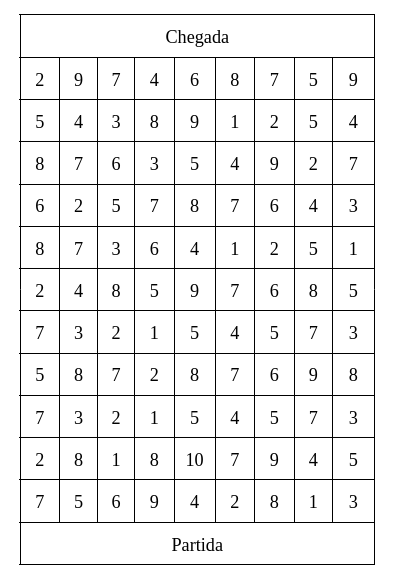
\includegraphics[width=0.4\linewidth]{img/tabuleiro}
	\caption{Tabuleiro do Zigue-Zague.}
	\label{tabuleiro-zigue-zague}
\end{figure}

O objetivo do jogo é alcançar a linha de chegada resolvendo expressões numéricas que envolvem adição e subtração. As regras utilizadas, como descritas em \cite{silvakodama:2007} e em \cite{unesp:2022}, são as seguintes:

\begin{enumerate}
	\item Todos os marcadores são colocados na linha de partida.
	\item Os jogadores se revezam (em alguma ordem) lançando os três dados.
	\item Em cada lançamento, o jogador deve realizar o cálculo de uma expressão numérica, envolvendo os números que foram obtidos no lançamento e as operações de adição e subtração, em qualquer ordem. Cada jogador deve comunicar as operações realizadas e o resultado aos demais jogadores.
	\item No primeiro movimento o jogador deverá colocar seu marcador em uma casa vaga da primeira linha, que contenha o resultado de sua expressão numérica.
	\item Nas demais jogadas, o jogador deverá deslocar seu marcador para a próxima linha, de acordo com o resultado de sua expressão numérica, desde que o valor obtido esteja em casa desocupada e vizinha (adjacente) à sua, na diagonal, horizontal ou vertical.
	\item Caso não seja possível movimentar seu marcador ou haja erro de cálculo (normalmente detectado pelo adversário), o jogador passa a vez.
	\item Vence o jogo quem primeiro alcançar a linha de chegada.
\end{enumerate}

O Projeto Zigue-Zague, por sua vez, se trata de uma pesquisa realizada pela Professora Evelize Aparecida dos Santos Ferracini (coordenadora do projeto), tendo os seguintes participantes: Professora Anne Raphaela Ledesma Cerqueira, Professor Valdiego Siqueira Melo e pelo estudante Michel Ferracini (autor deste artigo), todos do Instituto Federal de Educação, Ciência e Tecnologia de Mato Grosso, Campus Primavera do Leste. O projeto foi submetido e aprovado pelo EDITAL 09/2021 - PROIC - IFMT - PDL - FLUXO CONTÍNUO.

O objetivo geral do projeto é o estabelecimento de uma modelagem matemática (essencialmente probabilística) e computacional (implementada com a linguagem de programação \textit{Python}) do Zigue-Zague, para responder os seguintes questionamentos:

\begin{enumerate}
	\item Qual o total de caminhos no tabuleiro? (Onde \aspas{caminho} é qualquer sequência de 11 (onze) casas do tabuleiro, da primeira até a última linha, que se encadeiam de acordo com as regras do jogo.)
	\item Todos os caminhos possuem mesma chance de vitória?
	\item Existe alguma estratégia geral vencedora? Isto é, existe alguma estratégia baseada nos caminhos possíveis e na forma como se distribuem pelo tabuleiro que potencializa as chances de vitória?
\end{enumerate}

A pesquisa supracitada obteve os seguintes resultados:

\begin{enumerate}
	\item Implementou o código para calcular todos os possíveis caminhos no tabuleiro, obtendo como resultado 339 699 caminhos distintos.
	\item Definiu um experimento aleatório e um espaço amostral para o jogo, juntamente com o código para mostrar todos os distintos resultados do experimento aleatório e do espaço amostral.
	\item Construiu um espaço de probabilidades para o Zigue-Zague e o código para calcular a probabilidade de cada evento de interesse para o jogo, ou seja, a saída dos números que deve-se obter para efetuar uma jogada no tabuleiro.
	\item Obteve um modelo para os caminhos no tabuleiro (utilizando variáveis e vetores aleatórios) e uma definição consistente para realizar o cálculo das probabilidades dos caminhos (consistindo, em síntese, na multiplicação das probabilidades de cada casa pertencente a cada caminho).
	\item Implementou o código para atribuir probabilidades a cada casa do tabuleiro, bem como a construção de um tipo de \aspas{mapa} do tabuleiro.
	\item Realizou análise do tabuleiro, de acordo com a probabilidade de vitória de cada caminho, culminando em uma estratégia vencedora (isto é, obteve uma delimitação no tabuleiro de jogo, indicando o conjunto de casas que potencializa as chances de vitória).
\end{enumerate}

O relatório base do Projeto Zigue-Zague foi escrito em \textit{Jupyter Notebook}\footnote{\textit{Jupyter Notebook} é um tipo de documento interativo para código (em várias linguagens de programação), texto (com ou sem marcação - \textit{HTML} ou \textit{Markdown}), visualizações de dados e outras saídas.} e está disponível em \url{https://github.com/michel-ferracini/zigue_zague}.

\subsection{Problema de Pesquisa}

Apesar do trabalho bem sucedido do grupo de pesquisa, notou-se uma certa lentidão nos códigos desenvolvidos para descobrir uma estratégia vencedora para o jogo.

%Apesar do trabalho bem sucedido do grupo de pesquisa, notou-se uma certa lentidão nos códigos desenvolvidos para descobrir uma estratégia vencedora para o jogo, principalmente nos códigos de geração dos infográficos dos caminhos de mais alta e de mais baixa probabilidades e nas simulações de jogadas, utilizadas para confirmar estatisticamente a existência de uma região do tabuleiro onde as chances de vitória são potencializadas.  

A lentidão no processamento, mesmo não inviabilizando o estudo proposto, impede uma interação mais dinâmica com os dados obtidos, de modo que a busca por uma otimização do processamento, visando reduzir o tempo de execução dos códigos, torna-se desejável.

\subsection{Objetivos}
\label{objetivos}

Para resolver o problema observado, constitui-se os seguintes objetivos.


\begin{itemize}
	\item \textbf{Geral:} Avaliar o desempenho computacional dos códigos \textit{Python} utilizados no Projeto Zigue-Zague, visando reduzir o tempo de processamento.
	\item \textbf{Específicos:}
	\begin{enumerate}
		\item Realizar medições de tempo de execução nos códigos utilizados no Projeto Zigue-Zague.
		\item Encontrar hipóteses que expliquem o atual desempenho.
		\item Aplicar possíveis soluções de otimização de desempenho.
		\item Comparar os resultados de desempenho do projeto original com os novos resultados.
	\end{enumerate}
\end{itemize}

\subsection{Justificativa}
\label{justificativa}

O Projeto Zigue-Zague cumpriu os objetivos propostos, porém novos estudos podem ainda ser realizados, como apontado nas considerações finais do mesmo.

Além da existência de novas possibilidades ou interpretações no modelo de tabuleiro estudado, eventualmente utilizando diferentes bases teóricas (tanto na modelagem quanto na análise), há também uma certa variação de modelos de tabuleiros utilizados em aulas de Matemática, de modo que outros estudos baseados no Projeto Zigue-Zague podem seguir estratégias que requeiram um bom desempenho computacional para obter suas conclusões.

Em particular, sempre que for necessário gerar infográficos e realizar simulações ao estudar um tabuleiro de jogo, a questão do desempenho computacional inevitavelmente será colocada em discussão, pois a experiência e testes preliminares sugerem ser estes os processos mais lentos no estudo. Usando a função \aspas{mágica} \textit{\%\%time} do \textit{IPython}\footnote{\textit{IPython} é um interpretador interativo para várias linguagens de programação, mas especialmente focado em \textit{Python}.} em cada célula do \textit{notebook} do projeto e variando os dados para observação e análise, os resultados de tempo de processamento variaram de milissegundos até 10 minutos, sugerindo que cargas mais intensas de trabalho podem tornar a obtenção de resultados mais trabalhosa, quando não inviável. 

Mesmo para outros estudos, que apenas façam uso das técnicas apresentadas no projeto, mas não necessariamente tratem do jogo Zigue-Zague, torna-se relevante a busca por melhor desempenho computacional.

\subsection{Metodologia}
\label{metodologia}

Os procedimentos adotados neste trabalho são empíricos, especificamente guiados pela medição da variável tempo.

Usa-se o comando \aspas{mágico} \textit{\%timeit} do \textit{IPython} e os programas \textit{gprof2dot} e \textit{SnakeViz} para averiguar o tempo de execução em cada iteração de toda função do código, antes e após a implementação das seguintes estratégias:

\begin{enumerate}
	\item \label{reestruturacao} Reestruturação (ou refatoração) de códigos a partir de possíveis alterações em sua lógica.
	
	\item \label{substituicao} Substituição de códigos usando a biblioteca \textit{Python} \textit{NumPy}, comumente utilizada em computação científica.
	
	\item \label{decoradores} Utilização dos decoradores da biblioteca \textit{Python} \textit{Numba} nos gargalos encontrados com \textit{\%timeit} e com os programas \textit{gprof2dot} e \textit{SnakeViz}.
	
	\item \label{paralela} Utilização da opção de computação paralela, em iterações onde seja necessário percorrer todos os itens de um \textit{array}.
\end{enumerate}

O item \ref{reestruturacao} advém da percepção, apontada na Seção \ref{justificativa}, de que procedimentos cujos retornos sejam impressões em tela geram grande demanda de tempo de processamento. Assim, entende-se que a busca por redundâncias no processo e impressões desnecessárias que possam ser substituídas por cálculos ou reduzidas por análise estatística, sejam caminhos viáveis para atingir o objetivo proposto.

Já os itens \ref{substituicao}, \ref{decoradores} e \ref{paralela} são propostos pela natureza dos códigos do projeto, sempre envolvendo muitas interações com laços \textit{for}, de modo que cada uma das propostas sugeridas são viáveis, como fundamentado na Seção \ref{fundamentacao}. 

Para guiar este estudo, tomou-se como princípio as seguintes duas citações sobre otimização (traduzidas livremente), encontradas em \cite{hegde:2004}, um artigo sobre geração de perfis de programas:

\begin{itemize}
	\item \aspas{Mais pecados de computação são cometidos em nome da eficiência (sem necessariamente alcançá-la) do que por qualquer outro motivo - incluindo estupidez cega.} \textit{- -  William A. Wulf}\footnote{More computing sins are committed in the name of efficiency (without necessarily achieving it) than for any other single reason - including blind stupidity \textit{- -  William A. Wulf}}
	\item \aspas{Devemos esquecer as pequenas eficiências, digamos cerca de 97\% das vezes: a otimização prematura é a raiz de todos os males.} \textit{- -  Donald E. Knuth}\footnote{We should forget about small efficiencies, say about 97\% of the time: premature optimization is the root of all evil. \textit{- -  Donald E. Knuth}}
\end{itemize}

Buscou-se, neste estudo, seguir a linha de raciocínio expressa nas frases acima, de modo que não aplicou-se estratégias para melhoria de desempenho computacional em todo o código. Utilizou-se o comando mágico \textit{\%timeit} e os programas \textit{gprof2dot} e \textit{SnakeViz} para encontrar os gargalos no código e apenas em tais pontos executou-se as estratégias listadas no início desta seção.

%Em \cite{perkovic:2016}, ... Em \cite{oliveira:2015}, ... Em \cite{fernandez:2015}

%		Computação paralela. Ver Perkovic, seção 12.4 - Computação Paralela.
%		Sobre computação paralela, utlizar como referência Introdução à Ciência da Computação Usando Python (Seção 12.4, página 353).
%		Ver complexidade de algoritmos

%Ciência de Dados com Reprodutibilidade usando
%Jupyter - link https://sol.sbc.org.br/livros/index.php/sbc/catalog/download/67/292/544-1?inline=1

\section{Fundamentação Teórica}
\label{fundamentacao}

Nesta seção, realiza-se um detalhamento do ferramental utilizado neste estudo, como apresentado na Seção \ref{metodologia}. Assim, mostra-se a viabilidade teórica do trabalho de avaliação e melhoria de desempenho computacional propostos, indicando as bases tomadas como parâmetro para o mesmo.

% Comandos mágicos do IPython
\subsection{Comandos Mágicos do Interpretador IPython}

A fonte do texto desta subseção, exceto por pequenas adaptações de escrita, é \cite{mckinney:2018}.

%O \textit{IPython} é um importante recurso da pilha moderna de dados \textit{Python}, que apesar de não oferecer nenhuma ferramenta  de processamento ou de análise de dados, foi projetado desde o início para maximizar a sua produtividade, tanto
%em um processamento interativo, quanto no desenvolvimento de software. Ele incentiva um fluxo de trabalho de execução-exploração, em vez do fluxo de trabalho típico de edição-compilação-execução de muitas outras linguagens de programação.
%
%A equipe desenvolvedora do \textit{IPython} também desenvolveu o projeto \textit{Jupyter} (\url{http://jupyter.org/}), que é uma iniciativa mais ampla para projetar ferramentas de processamento interativas, independentes da linguagem. O \textit{notebook web} do \textit{IPython} passou a ser o \textit{notebook Jupyter}, com suporte hoje em dia para mais de 40 linguagens de programação. O sistema \textit{IPython} pode ser utilizado como um \textit{kernel} (um modo de linguagem de programação) para usar \textit{Python} com o \textit{Jupyter}. O \textit{shell IPython} e os \textit{notebooks Jupyter} são particularmente convenientes para exploração e visualização de dados.

O \textit{IPython} possui comandos especiais conhecidos como comandos \aspas{mágicos}, que servem para facilitar tarefas comuns e permitem controlar facilmente o comportamento do sistema \textit{IPython}. Um comando mágico é qualquer comando prefixado com o símbolo de porcentagem (\%), podendo ser visto como um programa de linha de comando para ser executado no sistema \textit{IPython}.

Por exemplo, para conferir o tempo de execução de qualquer instrução \textit{Python}, como uma multiplicação de matrizes, é possível utilizar a função mágica \textit{\%timeit}.

A instrução \textit{\%timeit}, executa uma instrução várias vezes para calcular um tempo médio de execução do conjunto; é útil para medir o tempo de um código cujo tempo de execução é muito rápido. 

% Programa gprof2dot
\subsection{Programa \textit{gprof2dot}}

%O programa \textit{gprof2dot}, criado por  José Fonseca e disponibilizado em sua conta no \textit{GitHub} em \url{https://github.com/jrfonseca/gprof2dot} (acesso em: 16 mai. 2022), foi desenvolvido (como descrito no README.md do projeto) para analisar o código de um programa, indicando quanto tempo cada parte do código precisa para ser executada. Também gera uma série de estatísticas relacionadas às chamadas de função no código.

O programa \textit{gprof2dot}, como descrito no \textit{README.md} do projeto no \textit{GitHub} \cite{fonseca:2022}, foi desenvolvido para analisar o código de um programa, indicando quanto tempo cada parte do código precisa para ser executada. Também gera uma série de estatísticas relacionadas às chamadas de função no código.

O programa sintetiza em um grafo as informações de desempenho do código em análise. Cada nó no grafo de saída representa uma função (ou método) e apresenta as seguintes informações: nome da função; porcentagem do tempo de execução gasto na função e em todos os seus filhos; porcentagem do tempo de execução gasto somente na função (entre parêntesis); total de vezes que a função foi chamada (incluindo chamadas recursivas). Cada aresta do grafo representa as chamadas entre duas funções e apresenta as seguintes informações: porcentagem do tempo de execução transferido dos filhos para o pai (se disponível); número de chamadas (de filhos) que a função pai realizou.

%Site útil: https://programming-techniques.com/ask-10549-how-can-you-profile-a-python-script/

%Comandos para gerar grafo:
%python3 -m cProfile -o profile.pstats main.py 
%gprof2dot -n 10 -f pstats profile.pstats | dot -Tsvg -o figura.svg
%

\subsection{Programa \textit{SnakeViz}}
%Comando para gerar visualização web do programa (é necessário já ter criado o arquivo .pstats acima):
%snakeviz profile.pstats

O programa \textit{SnakeViz}, como descrito em \cite{SnakeViz:2022}, é um visualizador gráfico baseado em navegador \textit{web} para a saída do módulo \textit{cProfile} do \textit{Python} e uma alternativa ao uso do módulo \textit{pstats} da biblioteca padrão\footnote{Segundo a documentação oficial do \textit{Python} \cite{python:2022}, \textit{cProfile} fornece perfis determinísticos de programas \textit{Python}, onde perfil é um conjunto de estatísticas que descreve com que frequência e por quanto tempo várias partes do programa são executadas. Essas estatísticas podem ser formatadas em relatórios por meio do módulo \textit{pstats}. O módulo \textit{cProfile} é uma extensão C com sobrecarga razoável que a torna adequada para criação de perfil de programas de longa duração.}. O \textit{SnakeViz} fornece informações sobre cada função do sistema em análise, indicando o tempo de execução acumulado para cada uma, o arquivo e a linha do arquivo onde se encontra a função. Além disso, é possível aplicar \textit{zoom} em cada componente do sistema para visualizar as chamadas internas para outras funções.

\textit{SnakeViz} tem dois estilos de visualização, \textit{icicle} (o padrão) e \textit{sunburst}. Em ambos a fração de tempo gasto em uma função é representada pela extensão de um elemento de visualização, seja a largura de um retângulo ou a extensão angular de um arco.

As funções não gastam apenas tempo chamando outras funções, elas também têm seu próprio tempo interno; o \textit{SnakeViz} mostra isso colocando um filho especial em cada nó que representa o tempo interno. Somente funções que chamam outras funções terão isso, funções sem chamadas são totalmente internas.

No estilo de visualização do \textit{icicle}, as funções são representadas por retângulos. Uma função raiz é o retângulo mais alto, com as funções que ela chama abaixo dele, depois as funções que elas chamam abaixo deles e assim por diante. A quantidade de tempo gasto dentro de uma função é representada pela largura do retângulo. Um retângulo que se estende pela maior parte da visualização representa uma função que está ocupando a maior parte do tempo de sua função de chamada, enquanto um retângulo fino representa uma função que quase não está sendo usada.
 
% Biblioteca NumPy
\subsection{Biblioteca \textit{NumPy}}

A fonte do texto a seguir, exceto por pequenas adaptações de escrita, novamente é \cite{mckinney:2018}.

\textit{NumPy} é uma abreviatura de \textit{Numerical Python} (ou Python Numérico), sendo um dos pacotes básicos mais importantes para processamento numérico em \textit{Python}. A maioria dos pacotes de processamento com funcionalidades científicas utiliza objetos \textit{array} do \textit{NumPy} como a \aspas{língua franca} para troca de dados.

Alguns dos recursos disponibilizados pelo \textit{NumPy} são:

\begin{itemize}
	\item ndarray: \textit{array} multidimensional eficaz, que oferece operações aritméticas rápidas, orientadas a \textit{arrays} e recursos flexíveis de \textit{broadcasting}.
	\item Funções matemáticas para operações rápidas em \textit{arrays} de dados inteiros, sem que seja necessário escrever laços.
	\item Ferramentas para ler ou escrever dados de \textit{array} em disco e trabalhar com arquivos mapeados em memória.
\end{itemize}

Um dos motivos para o \textit{NumPy} ser tão importante para processamentos numéricos em \textit{Python} é o fato de ele ter sido projetado para ser eficaz em grandes \textit{arrays} de dados. Há uma série de motivos para isso:

\begin{itemize}
	\item Internamente, o \textit{NumPy} armazena dados em um bloco contíguo de memória, independentemente de outros objetos \textit{Python} embutidos. A biblioteca do \textit{NumPy} de algoritmos escritos na linguagem C é capaz de atuar nessa memória sem qualquer verificação de tipo ou outro \textit{overhead}. Os \textit{arrays NumPy} também utilizam muito menos memória que as sequências embutidas de \textit{Python}.
	\item As operações do \textit{NumPy} realizam processamentos complexos em \textit{arrays} inteiros sem a necessidade de laços \textit{for} de \textit{Python}.
\end{itemize}

É importante notar que os algoritmos baseados no \textit{NumPy} geralmente são de 10 a 100 vezes mais rápidos do que suas contrapartidas em \textit{Python} puro, além de utilizarem significativamente menos memória.

% Biblioteca Numba
\subsection{Biblioteca Numba}
\label{numba}

O texto a seguir consiste em uma tradução livre e adaptada de parte da documentação oficial do \textit{Numba}, sendo \cite{numba:2022} a fonte original.

\textit{Numba} é um compilador \textit{just-in-time} para \textit{Python} que funciona melhor em código que usa matrizes e funções \textit{NumPy} e \textit{loops}. A maneira mais comum de usar o \textit{Numba} é através de sua coleção de decoradores que podem ser aplicados às suas funções para instruir o \textit{Numba} a compilá-las. Quando uma chamada é feita para uma função decorada com \textit{Numba}, ela é compilada para o código de máquina \aspas{\textit{just-in-time}} para execução e todo (ou parte do) seu código pode ser executado na velocidade do código de máquina nativa.

A utilização do \textit{Numba} é simples, não sendo necessário substituir o interpretador \textit{Python}, executar uma etapa de compilação separada ou até mesmo ter um compilador C/C++ instalado. Basta aplicar um dos decoradores do \textit{Numba} à função Python desejada e a biblioteca \textit{Numba} executa o processo automaticamente.

O \textit{Numba} será considerado uma boa escolha para melhorar o desempenho de um \textit{software} quando o código for orientado numericamente (faz muita matemática), usa muito o \textit{NumPy} ou tem muitos \textit{loops}.

% Computação paralela
\subsection{Computação Paralela}

O conceito de computação paralela advém da necessidade existente no mundo moderno de processar grandes quantidades de dados. Segundo \cite{perkovic:2016}, 

\citacao{Por várias décadas e até meados da década de 2000, os microprocessadores na maioria dos computadores pessoais tinham
	um único núcleo (ou seja, unidade de processamento). Isso significava que apenas um programa poderia ser executado de
	uma só vez nessas máquinas. A partir de meados daquela década, os principais fabricantes de microprocessador, como Intel
	e AMD, começaram a vender microprocessadores com várias unidades de processamento, normalmente chamados
	de núcleos (ou cores). Quase todos os computadores pessoais vendidos atualmente e muitos dispositivos sem fio possuem
	microprocessadores com dois ou mais núcleos.}

Para que o conceito de processamento paralelo seja entendido, é necessário primeiro esclarecer o conceito de processo. Em síntese, um processo é um \aspas{programa em execução}. Segundo \cite{perkovic:2016},

\citacao{Quando um programa é executado em um computador, ele é executado em um `ambiente' que registra todas as instruções de programa, variáveis, pilha de programa, o estado da CPU e assim por diante. Esse `ambiente' é criado pelo sistema operacional subjacente para dar suporte à execução do programa. Esse `ambiente' é aquilo que nos referimos como um processo.}

\noindent E continua explicando que 

\citacao{Os computadores modernos realizam multiprocessamento, o que significa que eles podem executar vários
	programas ou, mais precisamente, múltiplos processos simultaneamente. O termo simultaneamente não significa realmente `ao mesmo tempo'. Em uma arquitetura de computador com um multiprocessador de único núcleo, somente
	um processo pode estar realmente sendo executado em determinado momento. O que ele realmente significa neste
	caso é que, em qualquer ponto no tempo, existem vários processos (programas em execução), um dos quais está
	realmente usando a CPU e fazendo progresso; os outros processos são interrompidos, esperando que a CPU seja
	alocada a eles pelo sistema operacional. Em uma arquitetura de computador `multicore', a situação é diferente: vários
	processos podem verdadeiramente ser executados ao mesmo tempo, em núcleos diferentes.}

Usando a linguagem \textit{Python} é possível dividir a execução de um programa em várias tarefas. Uma possibilidade é utilizar o módulo \textit{multiprocessing} da Biblioteca Padrão para executar as diversas tarefas em paralelo por diferentes núcleos.

Outra possibilidade, em \textit{Python}, é a utilização do decorador para processamento paralelo disponível no interpretador \textit{Numba}, apresentado na Seção \ref{numba}.

\section{Resultados}

Para alcançar os objetivos propostos neste estudo, inicia-se na Subseção \ref{detalhamento} a avaliação do desempenho computacional do Projeto Zigue-Zague com uma descrição e análise da estrutura dos códigos gerados no projeto.

Em seguida, visando alcançar o primeiro objetivo (realizar medições de tempo de execução nos códigos utilizados no Projeto Zigue-Zague - ver Subseção \ref{objetivos}), é gerado na Subseção \ref{medicoes} um grafo de todo o programa e, também, usa-se o programa \textit{SnakeViz} para gerar uma visualização detalhada de cada parte do mesmo.

Na Subseção \ref{hipoteses} busca-se encontrar hipóteses que expliquem o atual desempenho dos códigos do projeto, partindo das medições de tempo de execução obtidas na subseção anterior.

No decorrer da Subseção \ref{solucoes}, são aplicadas soluções de otimização de desempenho, de acordo com as hipóteses formuladas na Subseção \ref{hipoteses}.

Finalmente, na Subseção \ref{comparacao}, os resultados de desempenho do projeto original são comparados com os novos resultados.

\subsection{Detalhamento do Código}
\label{detalhamento}

O Projeto Zigue-Zague possui três fases bem delimitadas: 

\begin{enumerate}
	\item modelagem matemática e computacional do tabuleiro de jogo; 
	\item geração de visualizações, que associam os caminhos de mais altas probabilidades e os de mais baixas com determinadas regiões do tabuleiro, culminando na observação de uma possível estratégia vencedora; 
	\item confirmação de uma estratégia vencedora a partir de simulações e análise estatística.
\end{enumerate} 

Em seguida, detalhes de cada uma destas fases são apresentados.

\subsubsection{Modelagem Matemática e Computacional}

A modelagem matemática e computacional, gerada na fase 1, é sintetizada em uma função (denominada \textbf{mapaTabuleiro}) que retorna uma lista (denominada \textbf{mapa\_tabuleiro}) contendo todos os 339 699 caminhos do tabuleiro, juntamente com as probabilidades de cada um destes caminhos. Cada elemento da lista é formado por um par - tupla - \textbf{(caminho, probabilidade do caminho)}. O primeiro elemento de \textbf{mapa\_tabuleiro} é o seguinte par:

\begin{lstlisting}[language=Python]
([[0, 0, 7, 0.04220779220779221], [1, 0, 2, 0.05844155844155844], 
	[2, 0, 7, 0.04220779220779221], [3, 0, 5, 0.05194805194805195],
	[4, 0, 7, 0.04220779220779221], [5, 0, 2, 0.05844155844155844], 
	[6, 0, 8, 0.03571428571428571], [7, 0, 6, 0.048701298701298704], 
	[8, 0, 8, 0.03571428571428571], [9, 0, 5, 0.05194805194805195], 
	[10, 0, 2, 0.05844155844155844]], 2.5159747913530996e-15)
\end{lstlisting}

%A Figura \ref{primeiro_elemento_mapeado} mostra o primeiro destes elementos, onde o \textbf{caminho} é uma lista de listas e a \textbf{probabilidade do caminho} é um \textit{float}.
%
%\begin{figure}[ht]
%	\centering
%	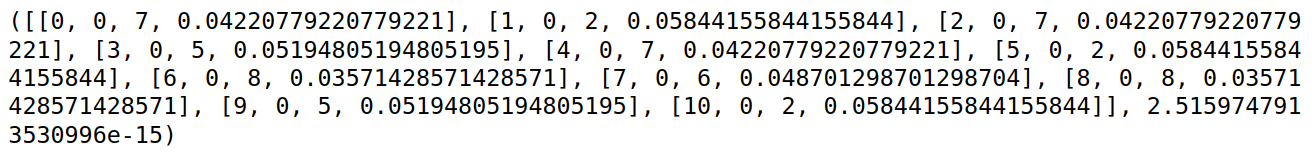
\includegraphics[width=1\linewidth]{img/primeiro_elemento_mapeado.png}
%	\caption{Primeiro elemento do mapeamento do tabuleiro.}
%	\label{primeiro_elemento_mapeado}
%\end{figure}

Melhor compreensão do elemento acima ilustrado, pode ser obtida na Figura \ref{explicacao_primeiro_elemento_mapeado}. O quadro da esquerda mostra os elementos do primeiro caminho, onde cada elemento é composto por um número entre 0 (zero) e 10 que indica a linha do tabuleiro, um número que pode variar de 0 (zero) a 8 e indica a coluna, um número que pode variar de 1 a 10 e indica o valor referente a casa do tabuleiro (que possui como coordenadas a linha e coluna marcadas nas posições anteriores) e um número entre 0 (zero) e 1 que indica a probabilidade do valor da casa ocorrer em um lançamento de dados. Já o quadro da direita mostra um número entre 0 (zero) e 1 que indica a probabilidade do caminho ocorrer.

\begin{figure}[ht]
	\centering
	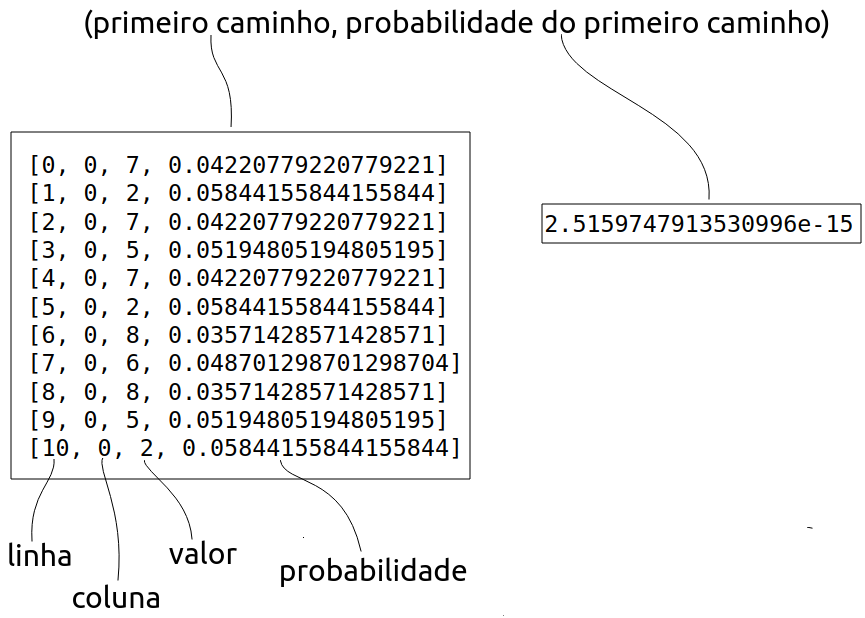
\includegraphics[width=0.8\linewidth]{img/explicacao_primeiro_elemento_mapeado.png}
	\caption{Detalhamento do primeiro elemento do mapeamento do tabuleiro.}
	\label{explicacao_primeiro_elemento_mapeado}
\end{figure}

A construção da função \textbf{mapaTabuleiro} utiliza diretamente outras três funções: \textbf{listaProximaJogada}, \textbf{tabProba} e \textbf{probaCaminho}, conforme ilustra a Figura \ref{construcao_mapaTabuleiro}.

\begin{figure}[ht]
	\centering
	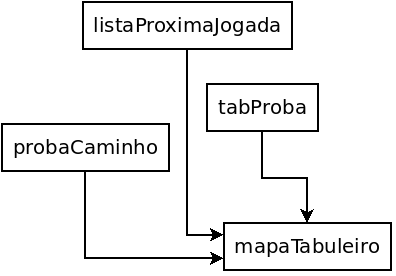
\includegraphics[width=0.45\linewidth]{img/construcao_mapaTabuleiro.png}
	\caption{Construção da função \textbf{mapaTabuleiro}.}
	\label{construcao_mapaTabuleiro}
\end{figure}

A função \textbf{listaProximaJogada} é construída para atender uma particularidade das regras do jogo: quando o jogador se encontra em um determinada posição no tabuleiro, suas possibilidades de avançar ficam restritas às casas adjacentes da linha superior. Já a função \textbf{tabProba} fornece à função \textbf{mapaTabuleiro} os valores das probabilidades de cada casa, de acordo com o valor da mesma. Por último, a função \textbf{probaCaminho} é utilizada para calcular o valor da probabilidade de cada possível caminho no tabuleiro.

A função \textbf{tabProba} também faz uso de funções auxiliares: \textbf{probabilidade} e \textbf{resultadoExpressoes}. De modo geral, o código para obtenção do mapeamento do tabuleiro faz uso de uma série de funções auxiliares, como mostra a Figura \ref{funcoes_auxiliares_mapaTabuleiro}, onde \textbf{produtoFiltrado} retorna todos os resultados possíveis no lançamento de três dados, \textbf{resultadoExpressoes} calcula e retorna os resultados de todas as possíveis expressões numéricas formadas com as possíveis configurações dos dados obtidas (com \textbf{produtoFiltrado}), \textbf{cardinalidade} retorna a cardinalidade de um evento simples do espaço amostral e \textbf{probabilidade} que retorna a chance de um evento ocorrer.

\begin{figure}[ht]
	\centering
	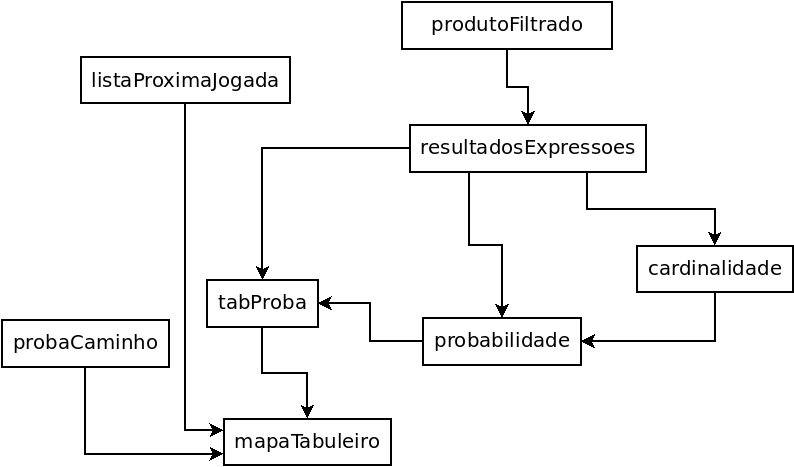
\includegraphics[width=0.9\linewidth]{img/funcoes_auxiliares_mapaTabuleiro.png}
	\caption{Diagrama mostrando a relação entre as funções utilizadas na modelagem matemática e computacional do tabuleiro.}
	\label{funcoes_auxiliares_mapaTabuleiro}
\end{figure}

\subsubsection{Visualizações}

As visualizações são geradas no Projeto Zigue-Zague especificamente pela função \textbf{imprimeCaminho}, que é chamada repetidas vezes para imprimir na tela cada caminho contido em qualquer submapa da lista \textbf{mapa\_tabuleiro}, obtida na fase 1 (descrita acima). A Figura \ref{funcoes_auxiliares_visualizacao} mostra as funções utilizadas no processo e suas inter-relações. A função \textbf{distintasProbas} percorre o mapeamento do tabuleiro (\textbf{mapa\_tabuleiro}) e retorna uma lista contendo apenas os distintos valores das probabilidades dos caminhos do tabuleiro. Já a função \textbf{configGraficos} é chamada no processo para criar um esquema de grade que representa o tabuleiro de jogo. A última função da Figura \ref{funcoes_auxiliares_visualizacao}, \textbf{mapaFaixaProbas}, percorre \textbf{mapa\_tabuleiro} comparando a probabilidade de cada caminho com dois valores, sendo o primeiro um valor mínimo de probabilidade e o segundo um valor máximo; quando a probabilidade de ocorrência de um caminho está entre o mínimo e o máximo informados, o caminho é anexado ao final de uma lista, que é então retornada pela função.

\begin{figure}[ht]
	\centering
	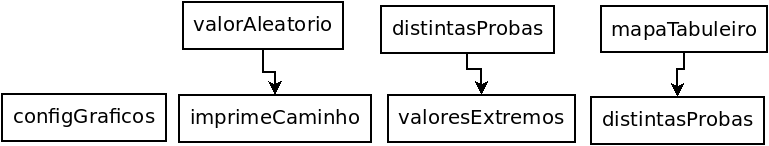
\includegraphics[width=0.8\linewidth]{img/funcoes_auxiliares_visualizacao.png}
	\caption{Diagramas das funções utilizadas no processo de visualização.}
	\label{funcoes_auxiliares_visualizacao}
\end{figure}

De modo geral, o código para gerar as visualizações utiliza as funções \textbf{mapaFaixaProbas}, \textbf{imprimeCaminho} e \textbf{configGraficos}, seguindo a seguinte estrutura: 

\begin{itemize}
	\item Primeiro a função \textbf{mapaFaixaProbas} é chamada duas vezes para criar um submapa inferior (\textbf{submapa\_inferior}) dos caminhos que possuem as 1000 menores probabilidades e, depois, para criar um submapa superior (\textbf{submapa\_superior}) dos caminhos com as 1000 maiores probabilidades:
	\begin{lstlisting}[language=Python]
	submapa_inferior = mapaFaixaProbas(
										mapa_tabuleiro, 
										distintas_probas, 
										0, 
										999)
	submapa_superior = mapaFaixaProbas(
										mapa_tabuleiro, 
										distintas_probas, 
										22076, 
										23076)
	\end{lstlisting}
	\item Na sequência um laço \textit{for} percorre \textbf{submapa\_superior} e usa a função \textbf{imprimeCaminho} para imprimir cada caminho:
	\begin{lstlisting}[language=Python]
	for caminho in submapa_superior:
		imprimeCaminho(caminho, 1, 'green')
	\end{lstlisting} 
	\item O mesmo é feito para \textbf{submapa\_inferior}:
	\begin{lstlisting}[language=Python]
	for caminho in submapa_inferior:
		imprimeCaminho(caminho, 1, 'red')
	\end{lstlisting}
	\item Finalmente a função \textbf{configGraficos} é chamada para exibir as impressões na tela, como mostra a Figura \ref{primeira_visualizacao}.
	\begin{figure}[ht]
		\centering
		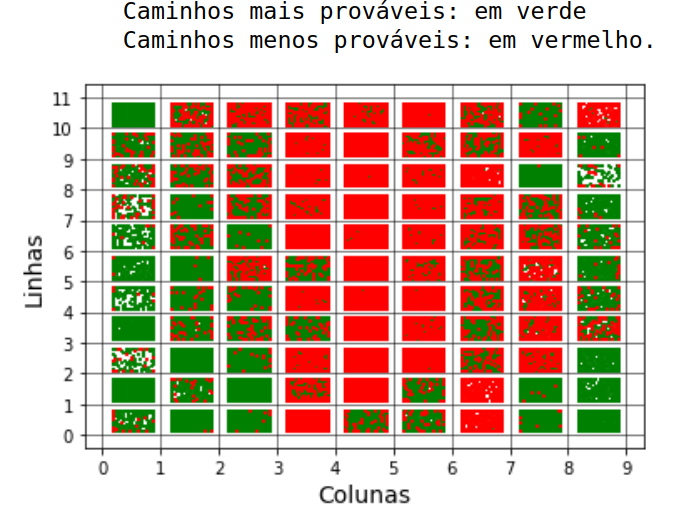
\includegraphics[width=0.7\linewidth]{img/primeira_visualizacao.png}
		\caption{Primeira visualização do Projeto Zigue-Zague.}
		\label{primeira_visualizacao}
	\end{figure}
\end{itemize}

A Figura \ref{primeira_visualizacao} é um importante resultado no projeto Zigue-Zague. Além dessa visualização, uma outra também é gerada, mas apenas invertendo a ordem de impressão das faixas de probabilidades. As imagens geradas servem para visualizar as regiões com as menores probabilidades de avançar no tabuleiro (indicadas com pontos vermelhos) e as regiões com as mais altas probabilidades de avançar (indicadas com pontos verdes).

\subsubsection{Confirmação de uma Estratégia Vencedora}

No texto do Projeto Zigue-Zague, é descrita a seguinte estratégia:

\citacao{No tabuleiro, as três colunas da esquerda (1, 2 e 3) constituem a região com maior probabilidade de avançar em um jogo; as três colunas centrais (4, 5 e 6) constituem a região com menor probabilidade; as três colunas da direita (7, 8 e 9) constituem uma região intermediária.

Enfim, jogar pela esquerda potencializa as chances de vencer no Zigue-Zague; a segunda melhor opção é avançar pela direita; a pior região é a central.}

Para confirmar que a região esquerda possui a maior chance de vitória é criada a função \textbf{jogar}, que simula as jogadas de um único jogador avançando do início até o fim em um tabuleiro, de acordo com as regras do jogo. A função \textbf{jogar} é então chamada repetidamente na função \textbf{simulacao}. A Figura \ref{confirmacao_regiao_vencedora} mostra a inter-relação das funções utilizadas para gerar as simulações.

\begin{figure}[ht]
	\centering
	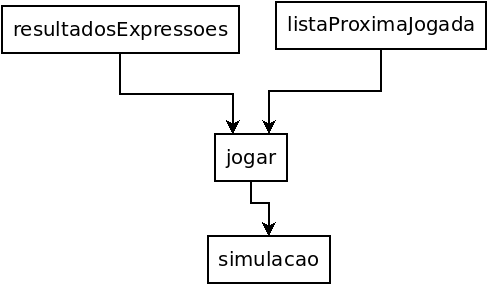
\includegraphics[width=0.55\linewidth]{img/confirmacao_regiao_vencedora.png}
	\caption{Diagrama das funções utilizadas para confirmar uma estratégia vencedora.}
	\label{confirmacao_regiao_vencedora}
\end{figure}

A função \textbf{jogar} recebe como parâmetro um tabuleiro reduzido (com 3 colunas), retornando a quantidade de jogadas
em que não foi possível avançar por falta de opção. O código passa pelas seguintes etapas:

\begin{itemize}
	\item Escolhe uma coluna (na faixa determinada para a simulação) aleatoriamente.
	\item Entra em um laço para percorrer cada linha do tabuleiro.
	\item \aspas{Lança} os dados.
	\item Calcula todas as possíveis expressões para os dados sorteados.
	\item Verifica as casas da próxima linha para confirmar se existem valores condizentes com as possíveis expressões.
	\item Se houver possibilidades de avançar, escolhe uma das casas disponíveis e realiza a jogada; caso contrário, contabiliza a tentativa, isto é, adiciona 1 à variável de retorno.
\end{itemize}

Finalmente, a função \textbf{simulacao} recebe como parâmetro o número de simulações desejadas e retorna uma terna - tupla - contendo a média do número de vezes (para cada entrada da terna) em que não houve opções de jogadas em cada região do tabuleiro (esquerda, centro e direita). 

Por exemplo, para a chamada \textbf{simulacao(2000000)} um possível retorno é a terna $(9.020566 , 11.190417 ,  9.6818985)$, indicando que na região esquerda houve em média $9.020566$ jogadas sem opções para avançar, na região central houve em média $11.190417$ jogadas e na região direita $9.6818985$.

No total, são realizadas 16 milhões de simulações, de 2 em 2 milhões.

\subsection{Medições no Tempo de Execução}
\label{medicoes}

Na geração do grafo (utilizando o programa \textit{gprof2dot}), foi estabelecida uma poda de todos os ramos que utilizam 10\% ou menos do tempo de processamento, como ilustrado na Figura \ref{grafo:10}.

\begin{figure}[ht]
	\centering
	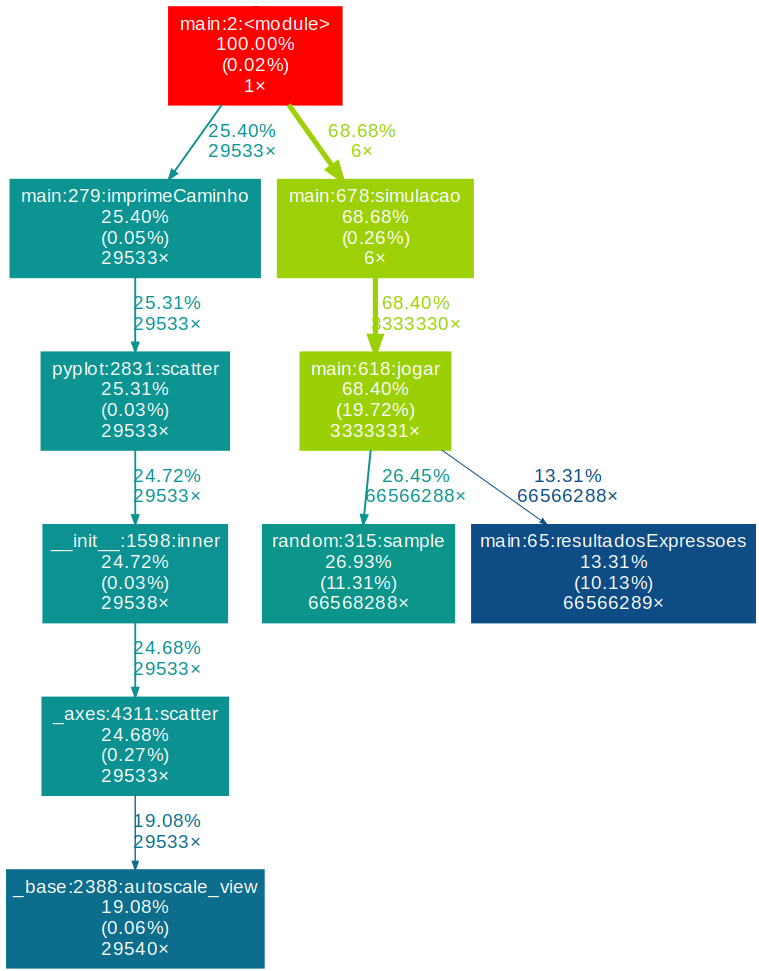
\includegraphics[width=0.7\linewidth]{img/grafo.png}
	\caption{Grafo do programa, com poda para 10\% ou menos do tempo de processamento, gerado com o programa \textit{gprof2dot}.}
	\label{grafo:10}
\end{figure}

No lado esquerdo do grafo (Figura \ref{grafo:10}), a função \textbf{imprimeCaminho} possui como filho o método \textbf{scatter} do módulo \textit{pyplot} da biblioteca \textit{matplotlib}, sendo chamado todas as vezes que se faz necessário imprimir um ponto na geração da visualização dos caminhos de mais alta probabilidades e também dos de mais baixas probabilidades no tabuleiro de jogo. No lado direito, a função \textbf{simulação} chama repetidamente a função filha \textbf{jogar} que, por sua vez chama repetidamente dois filhos: o método \textbf{sample} da biblioteca \textit{random} e a função \textbf{resultadosExpressoes}.

Na visualização gerada com o \textit{SnakeViz} (Figura \ref{viewSnakeViz}), observa-se a mesma configuração de uso do tempo de processamento. Em particular, o tempo de uso de cada função aparece na visualização. Com relação ao grafo na Figura \ref{grafo:10}, a função \textbf{resultadosExpressoes} é a única que não aparece, mas aplicando \textit{zoom} torna-se possível observar essa informação, como mostra a Figura \ref{viewSnakeVizZoom}.

\begin{figure}[ht]
	\centering
	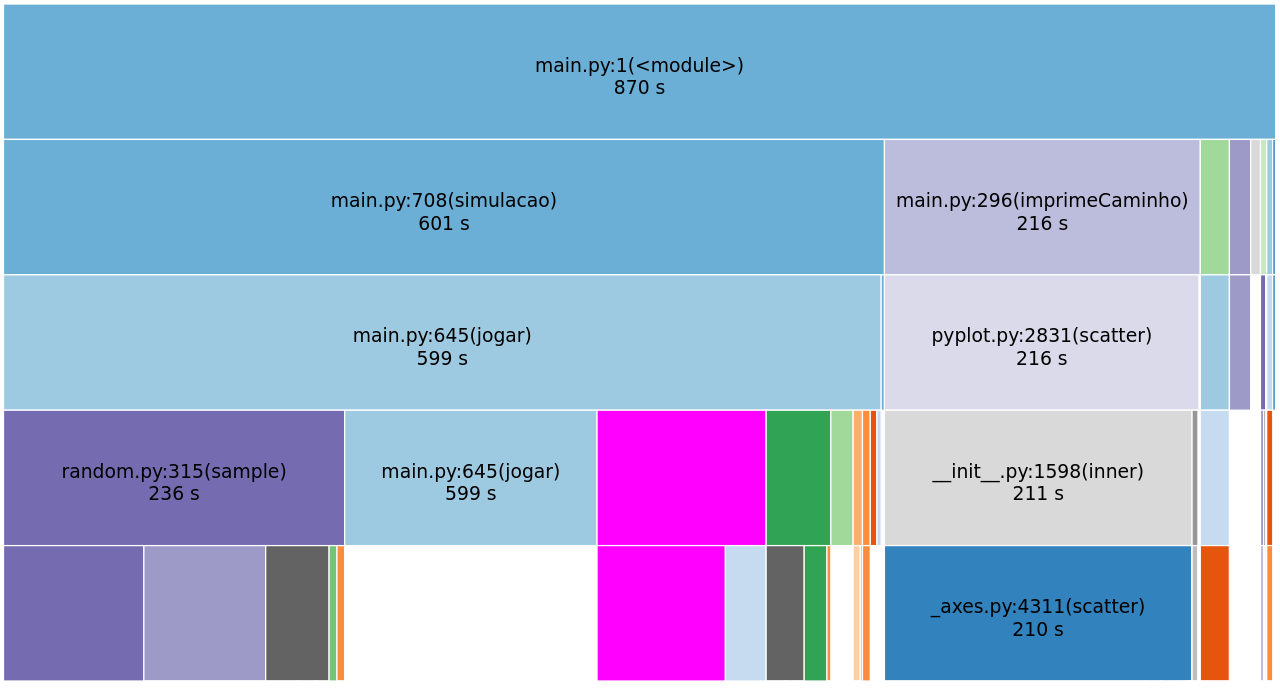
\includegraphics[width=0.9\linewidth]{img/view_snakeviz_1.png}
	\caption{Visualização gerada com o \textit{SnakeViz}.}
	\label{viewSnakeViz}
\end{figure}

\begin{figure}[ht]
	\centering
	
\includegraphics[width=0.9\linewidth]{img/viewSnakeVizZoom.png}
	\caption{\textit{Zoom} para visualizar a função \textbf{resultadosExpressoes}.}
	\label{viewSnakeVizZoom}
\end{figure}

O grafo foi utilizado apenas para permitir melhor visualização da relação entre as funções, enquanto os dados de tempo de processamento (e, consequentemente, do percentual) utilizados neste artigo são provenientes da visualização gerada pelo \textit{SnakeViz}. O resumo destas informações do programa são mostrados na Tabela \ref{tab}, onde a coluna \textbf{Função} estabelece o nome da função chamada, a coluna \textbf{Número de chamadas} mostra a quantidade de vezes que uma função foi chamada durante toda a execução do programa, a coluna \textbf{Tempo acumulado} exibe a soma de todas as chamadas de uma função e a coluna \textbf{Percentual} fornece o percentual de tempo gasto na execução de determinada função com relação ao tempo total de execução, correspondente à função \textbf{main}.

\begin{table}[H]
	\centering
	\caption{Resumo da medição dos tempos de execução do programa.}
	\label{tab}
	\begin{tabular}{|m{0.07\linewidth}|m{0.25\linewidth}|m{0.15\linewidth}|m{0.21\linewidth}|m{0.17	\linewidth}|}
		\hline
		 & \textbf{Função} & \textbf{Número de chamadas} & \textbf{Tempo acumulado (segundos)} & \textbf{Percentual}\\
		\hline \hline
		1 & \textbf{main} & $1$	& $2,08 \cdot 10^4$ & $100$ \\
		\hline
		1.1 & \textbf{simulacao} & $8$	& $1,71 \cdot 10^4$  & $82,07$ \\
		\hline
		1.1.1& \textbf{jogar} & $48000001$ & $1,70 \cdot 10^4$ & $81,69$ \\
		\hline
		1.1.1.1 & \textbf{sample} & $958276283$ & $6,60 \cdot 10^3$ & $31,68$ \\
		\hline
		1.1.1.2 & \textbf{resultadosExpressoes} & $958276284$ & $3,28 \cdot 10^3$ & $15,75$ \\
		\hline
		1.2 & \textbf{imprimeCaminho} & $69267$   & $3,70 \cdot 10^3$ & $17,76$ \\
		\hline
		1.2.1 & \textbf{scatter} & $69267$ & $3,70 \cdot 10^3$ & $17,74$ \\
		\hline
	\end{tabular}
\end{table}

Da análise realizada nesta subseção, conclui-se que as funções listadas na Tabela \ref{tab} são as mais relevantes para o desempenho dos códigos no projeto Zigue-Zague. O tempo total de execução do código foi igual a $2,08 \cdot 10^4$ segundos, o que corresponde a 5 horas, 46 minutos e 40 segundos. Na próxima subseção, esta tabela direciona fortemente a busca por hipóteses que expliquem o desempenho dos códigos do projeto.

\subsection{Formulação de Hipóteses}
\label{hipoteses}

Seção referente ao objetivo específico:\\
Encontrar hipóteses que expliquem o atual desempenho.

\subsection{Aplicação de Possíveis Soluções}
\label{solucoes}

Seção referente ao objetivo específico:\\
Aplicar possíveis soluções de otimização de desempenho.

\subsection{Comparação de Desempenho}
\label{comparacao}

Seção referente ao objetivo específico:\\
Comparar os resultados de desempenho do projeto original com os novos resultados.

% Referências (apenas o que for citado no texto com \cite{})
\bibliographystyle{sbc}
\bibliography{sbc-template}

\end{document}
